\documentclass{examen}

\begin{document}
\modulo{Lenguajes de marcas -- PARTE ESCRITA (PARTES 1 y 2)}

\pregunta{Crear en HTML un formulario como el mostrado en la figura.}{2}
\begin{figure}[h]
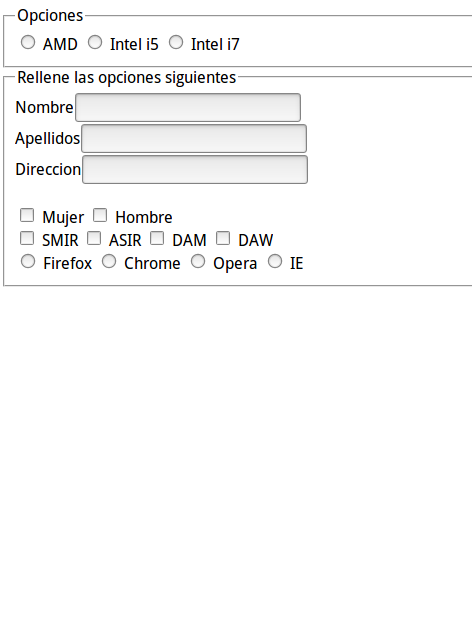
\includegraphics[scale=0.5]{examen-img/foto_formulario_11.png}
\end{figure}
\break


\pregunta{Elaborar un esquema XML que permita validar un fichero XML que se atenga a las reglas siguientes:}{3.5}
\begin{itemize}

\item{El elemento ra�z se llama {\tt ficheros}. Dentro de �l debe haber 0 o m�s elementos {\tt fichero}. Dentro de {\tt fichero }
debe haber un elemento {\tt creador} y puede haber o no un {\tt tamanio }. El elemento {\tt fichero} debe llevar siempre un atributo obligatorio ``creacion'' y la estructura de ese atributo es AAAA-MM-DD.}

\item{Un {\tt creador} debe llevar un atributo obligatorio llamado {\tt grupo}. Dentro de {\tt grupo} puede haber cualquier cadena. Dentro del elemento {\tt creador} solo puede haber los usuarios ``usu01'' o ``usu02''}.
\item{El elemento {\tt tamanio} es optativo. Si aparece debe llevar obligatoriamente un atributo ``unidad''. Dentro de dicho atributo ``unidad'' solo puede haber {\tt bytes} o {\tt megabytes}. Dentro de {\tt tamanio} debe haber un entero positivo.}
\end{itemize}

\begin{verbatim}
<!--Ejemplo de fichero para los ejercicios-->
<ficheros> <!--Elemento ra�z-->
    <!--Hay 0 o m�s elementos fichero. "Creacion" es obligatorio-->
    <fichero creacion="2019-02-01">
        <!--Elemento "creador" obligatorio. Atributo "grupo"
        obligatorio. Dentro de "creador" solo puede haber "usu01"
        o "usu02"-->
        <creador grupo="root">usu01</creador>
        <!--Tamanio es un elemento optativo. El atributo
        unidad es obligatorio y solo puede ser
        "bytes" o "megabytes".Dentro de tamanio solo
        hay un entero positivo, en este caso 281-->
        <tamanio unidad="bytes">281</tamanio>
    </fichero>
    <fichero creacion="2019-03-03">
        <creador grupo="usuarios">usu02</creador>
    </fichero>
    <fichero creacion="2019-03-03">
        <creador grupo="root">usu02</creador>
    </fichero>
</ficheros>
\end{verbatim}
\end{document}
